%!TEX root = ../adventure.tex

\chapter{Prolog}
\label{adventure}

\begin{advquote}
\large Sieh dich vor, Gevatter Tod ist auf dem Weg zu dir. Und auch zu mir.
\end{advquote}

Wir schreiben das Jahr 1350. Hamburg wächst dank des erstarkenden Seehandels stetig
und die Hanse trägt ihren Teil dazu bei. Täglich gehen am Rheinhafen Schiffe aus
aller Herren Länder vor Anker, während vom Rathaus an der Troßtbrücke der Rat die
Geschicke der Stadt lenkt. Es ist eine Zeit des Aufbruchs, aber auch eine Zeit der
Angst. Denn neben Piraten und anderen finsteren Gestalten, die zunehmend in den
Gassen der Stadt umherstreifen, greift etwas noch viel gefährlicheres um sich. Die
Leute hatten bereits von einem „Schwarzen Tod" gehört, der binnen weniger Tage einen
gesunden Mann seiner Lebenskraft zu berauben vermag. Nun scheint es so, als sei die
Plage auch in die Wohnungen von Hamburg eingedrungen. Der düstere Geruch des Todes
zieht durch die Docks, während der Rat darüber entscheidet, was zu tun ist.

Und was auch immer das sein mag, es muss schnell geschehen.
\vspace{0.7cm}

\section{Im Wartezimmer des Rathauses}
\label{sec:wartezimmer}

So begibt es sich, dass ihr geduldig vor einer gewaltigen Holztür im Ratshaus an der
Troßtbrücke sitzt. Am gestrigen Abend wurdet ihr von Boten aufgesucht, die euch baten
am folgenden Tag vor dem Hamburger Rat zu erscheinen, zu den man euch nun in wenigen
Augenblicken rufen wird. Noch besteht etwas Zeit sich zu unterhalten und umzusehen.

\vspace{0.3cm}

\begin{tcolorbox}

\vspace{0.7cm}
\centering\textbf{Raumbeschreibung}

\flushleft
Die Gruppe sitzt in einer Art Warteraum, der für damalige Verhältnisse sehr üppig
eingerichtet ist. Es hängen mehrere Bilder von großen Hamburger Persönlichkeiten an
den Wänden. Außerdem stehen kleine exotische Leckereien bereit, und auch Getränke
werden angeboten. In einer Ecke des Raumes steht ein Ratsdiener. An der Wand hängt
eine Karte der Stadt, welche die Charaktere sich ansehen können. Diese wird den
Spielern im weiteren Verlauf des Abenteuers auch zur Verfügung stehen.
\end{tcolorbox}

\begin{figure}[t]
\begin{center}
	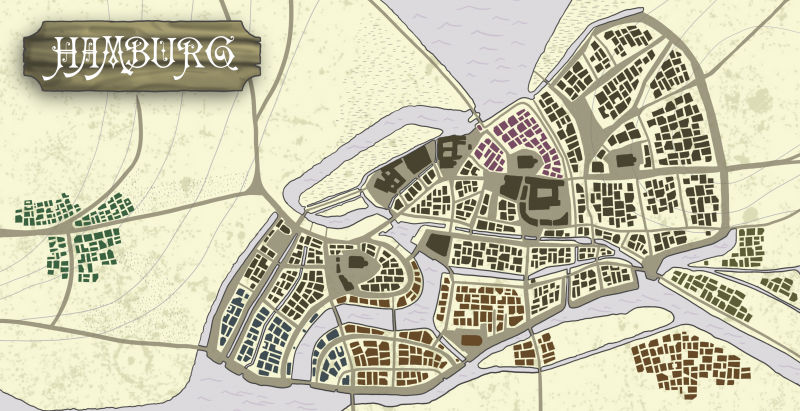
\includegraphics[scale=0.7]{./01-img/Karte.png}
	\caption{Stadkarte von Hamburg, anno 1350}
    	\label{fig:Karte}
\end{center}
\end{figure}


\section{Das Gespräch mit dem Rat}
\label{sec:ratsgespräch}

Als Ihr euch also unterhaltet öffnet sich plötzlich die Holztür und ein junger
Ratsdiener bittet euch vor den Rat zu treten.

\textbf{Raumbeschreibung}: Ihr tretet in einen großen Raum ein, der von einer U-förmigen Tischreihe dominiert wird und an dem 18 Männer in erhöhter Position sitzen. Auch wenn der Raum sonst nur spärlich eingerichtet ist, ist offensichtlich dass sich hier sonst niemand aufhält, der wenig Geld hat. Aus den Wänden sind kunstvoll Löwenköpfe und andere Muster herausgearbeitet. Eine Wand ist von hohen Fenstern gesäumt, die den Raum hell erleuchten.

Im Hintergrund huschen Ratsdiener mit Papieren umher oder gehen anderen Aufgaben nach.

%\red{\textbf{Info}: Die 18 Männer setzen sich aus neun Rechtskundigen, sieben Kaufleuten und zwei Vertretern der Kirche zusammen.}
%\newpage
%\red{\textbf{Interaktion}}:

Vorsitzender des Rates:
%\gqm{\textit{Der Hamburger Rat dankt euch für euer Erscheinen. Bevor wir uns jedoch mit den euch betrauten Aufträgen befassen werden, sagt, was wisst ihr über die Pestilenz?}}

%\red{\textbf{Probe auf Gesellschaft/Wissen o.Ä}: Menschen die von der Pestilenz befallen sind leiden unter Schwindelgefühlen und Schüttelfrost. Auch klagen manche über starke Kopfschmerzen und erbrechen sich häufig. Ein hohes Fieber sowie schwarze Pestbeulen an den Lymphknoten treten im Verlaufe der Krankheit auf und sind für den Patienten meist ein sicheres Todeszeichen.}

%\red{\textbf{kritischer Erfolg/Probe auf Medizin}: Manche Heiler berichten, dass sie die Pestbeulen aufschneiden und vom darin enthaltenden Eiter reinigen. Wird anschließend das Fieber eines Kranken behandelt konnte mancher Totgeglaubte wieder von der Pest geheilt werden.}

%Vorsitzender des Rates:
%\gqm{\textit{Nun ist dem Rat zu Ohren gekommen, dass auch vor den Mauern Hamburgs die Pestilenz ihr Unwesen treibt. Diese Krankheit muss so kurz vor dem christlichsten aller Feiertage unter allen Umständen aus der Stadt verdrängt werden. Zu diesem Zwecke werdet ihr in einen Beirat gerufen. Der Rat fordert euch auf in den nächsten vier Tagen die Fälle von Pestilenz zu untersuchen und dem Rat am fünften Tag eine Empfehlung auszusprechen, wie die Pestilenz zu bewältigen ist.}}

%\gqm{\textit{Werdet ihr eure Aufgaben gewissenhaft erfüllen soll es euer Schaden nicht sein. Außerdem werdet ihr während eurer Mitgliedschaft im Beirat in einer Kapelle nahe der St. Michaelis Kirche untergebracht werden, die fortan als eure Operationszentrale dienen wird, alle weiteren Informationen wird man dort für euch bereitlegen.}}

Anschließend wendet sich der Vorsitzende des Rates seinen Aufzechnungen zu. Unter den anderen Ratsmitgliedern keimen Gespräche auf, an den Spielern besteht nun für den Rat keine weitere Interesse. Sollten sich die Abenteurer nicht aus dem Raum zurückziehen werden sie nach einigen Momenten von Ratsdienern dazu aufgefordert.
